\section{Примеры} 
Положим, что матрица выигрышей двух игроков соответсвует~(\ref{table:sec:ot:real})
$r^g= 4 $ - количество ходов совершаемое  правительством за игру\\
$q^g =[ 0.5; 0.9; 0.7; 0.4 ]$ - соответсвующая скалярная функция \\
$r^p= 3 $ - количество ходов совершаемое  обществом за игру\\
$q^p=[ 0.6; 0.8; 1] $ - соответсвующая скалярная функция \\

\begin{figure}[h]
	
	\begin{subfigure}{0.5\textwidth}
		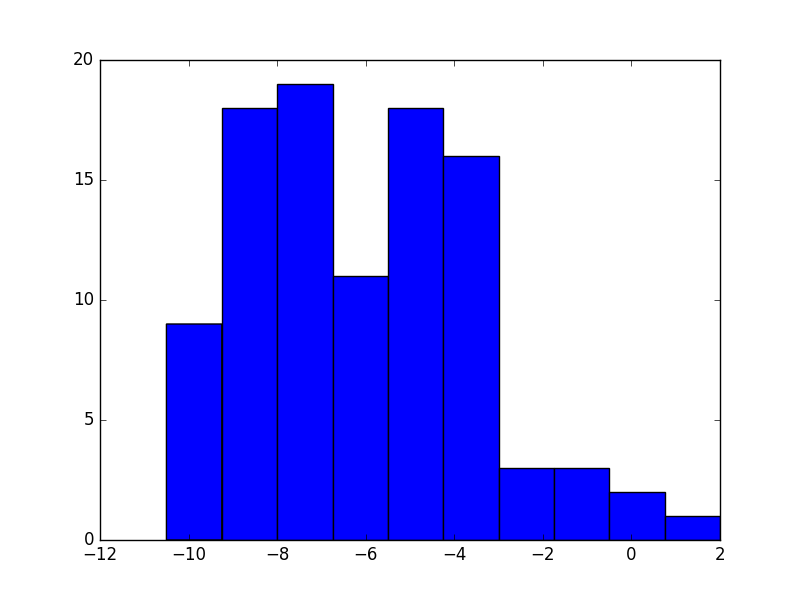
\includegraphics[width=0.9\linewidth]{Government1.png} 
		\caption{Правительство}
		\label{fig:government1}
	\end{subfigure}
	\begin{subfigure}{0.5\textwidth}
		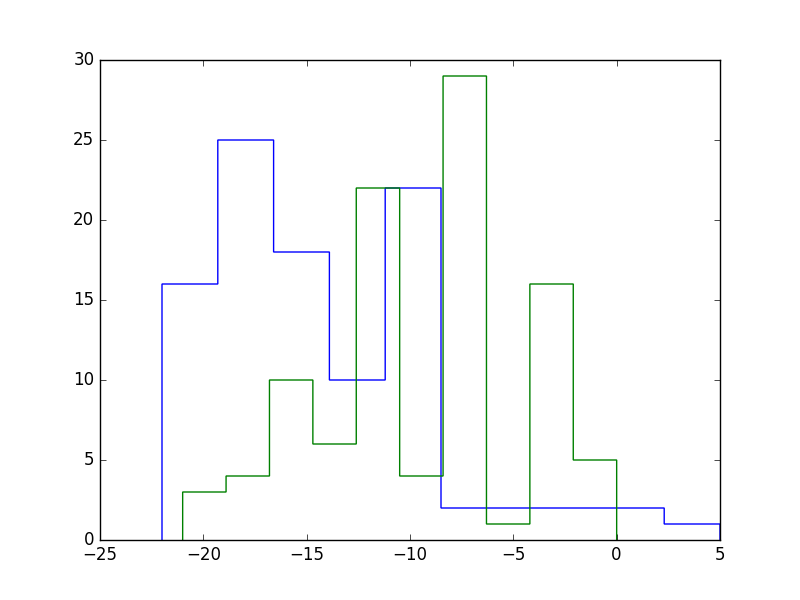
\includegraphics[width=0.9\linewidth]{Public1.png}
		\caption{Общественность}
		\label{fig:public2}
	\end{subfigure}
	
	\caption{Гистограмма выигрышей}
	\label{fig:stat1}
\end{figure}
Government's average = -4.55\\
Government's standard deviation = 2.86749019179\\
Government's asymmetry = -0.41010602681026553\\
Government's excess = 0.9969338499220726\\
Public's average = -6.1\\
Public's standard deviation = 2.21133443875\\
Public's asymmetry = -0.31057123429132594\\
Public's excess = -0.977347391965933\\

Тут будут какие-то выводы из статистических результатов и 2 примера, когда каждый по очереди следует проигрышной стратегии.
